
    \begin{abstract_online}{Role of Translational Jump-diffusion in the Breakdown of the Stokes-Einstein Relation in Supercooled Water and its Binary Mixture with Glycerol}{%
        \underline{S. Dueby}, S. Daschakraborty}{%
        }{%
        Department of Chemistry, IIT Patna, Bihar 801106, India}
    Several experiments have witnessed increasing violation of the Stokes-Einstein (SE) relation, connecting the translational self-diffusion and viscosity, in supercooled water and its mixture with different cosolvents, like glycerol, as the temperature decreases. Earlier studies explained the breakdown of the SE relation in terms of the location of the Widom line, emanating from the liquid-liquid critical point (LLCP). Although these studies made a significant contribution to understand the above phenomena, a detailed molecular picture is still lacking. Recently our group has been able to explain the SE breakdown from jump-diffusion approach [1-3]. The jump-diffusion coefficient — emanating from jump translation of water molecules — is calculated quantitatively for different temperature and pressure conditions. It is observed that the jump-diffusion is the key factor for the SE breakdown in supercooled water. The same method is adopted in the present work to explain the similar behavior in water/glycerol binary mixture at different temperatures. \begin{center}  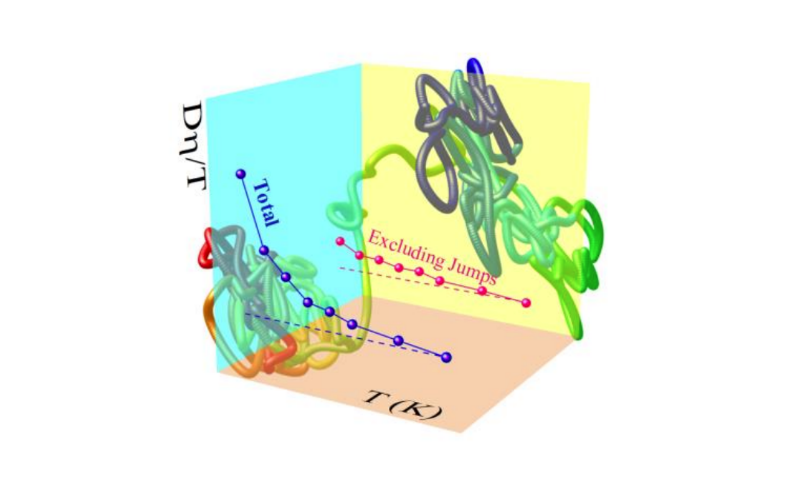
\includegraphics[width=0.8\linewidth]{abstracts/txt/figures/dueby.png}  \end{center}  
    
        \textbf{References} \newline{}[1] Dubey, V.; Erimban, S.; Indra, S.; Daschakraborty, S. Understanding the Origin of the Breakdown of the Stokes-Einstein Relation in Supercooled Water at Different Temperature-Pressure Conditions. J. Phys. Chem. B 2019, DOI: 10.1021/acs.jpcb.9b08309 (Just Accepted).\newline{}[2] Dueby, S.; Dubey, V.; Daschakraborty, S. Decoupling of Translational Diffusion from the Viscosity of Supercooled Water: Role of Translational Jump Diffusion. J. Phys. Chem. B 2019, 123 (33), 7178–7189.\newline{}[3] Dubey, V.; Kumar, N.; Daschakraborty, S. Importance of Solvents’ Translational– Rotational Coupling for\newline{}Translational Jump of a Small Hydrophobic Solute in Supercooled Water. J. Phys. Chem. B 2018, 122 (30),\newline{}7569–7583.
    \end{abstract_online}
    